\section{Chirality}
Chirality is an important concept which describes the ``handedness'' of the coordinate system. Even though we are restricted to $\real{2}$ in this discussion, we will see that we need to embed this plane in a third dimension. This is because we will see that we are either looking down on the plane (right thumb up) or looking \emph{up} at the plane (left thumb up). We color objects in the plane with a magic paint which is green from above and red from below. This will help us to keep track of the chirality. The axis in the $\hat{e}_{1}$ direction is black. The axis in the $\hat{e}_{2}$ direction is blue. We measure the angle from the $\hat{e}_{1}$ vector to the $\hat{e}_{2}$ in the plane which contains them. (In higher dimension we go from $\hat{e}_{k}$ vector to the $\hat{e}_{k+1}$.)

Here we go from black to blue. Run your fingers along the black line. If they curl in the direction of the blue line, the system is \emph{right handed.} If you must use your left hand fingers to curl in the direction of the blue line then the system is \emph{left-handed.}

\begin{table}[htdp]
\begin{center}
\begin{tabular}{l|ll}
 coordinate system & 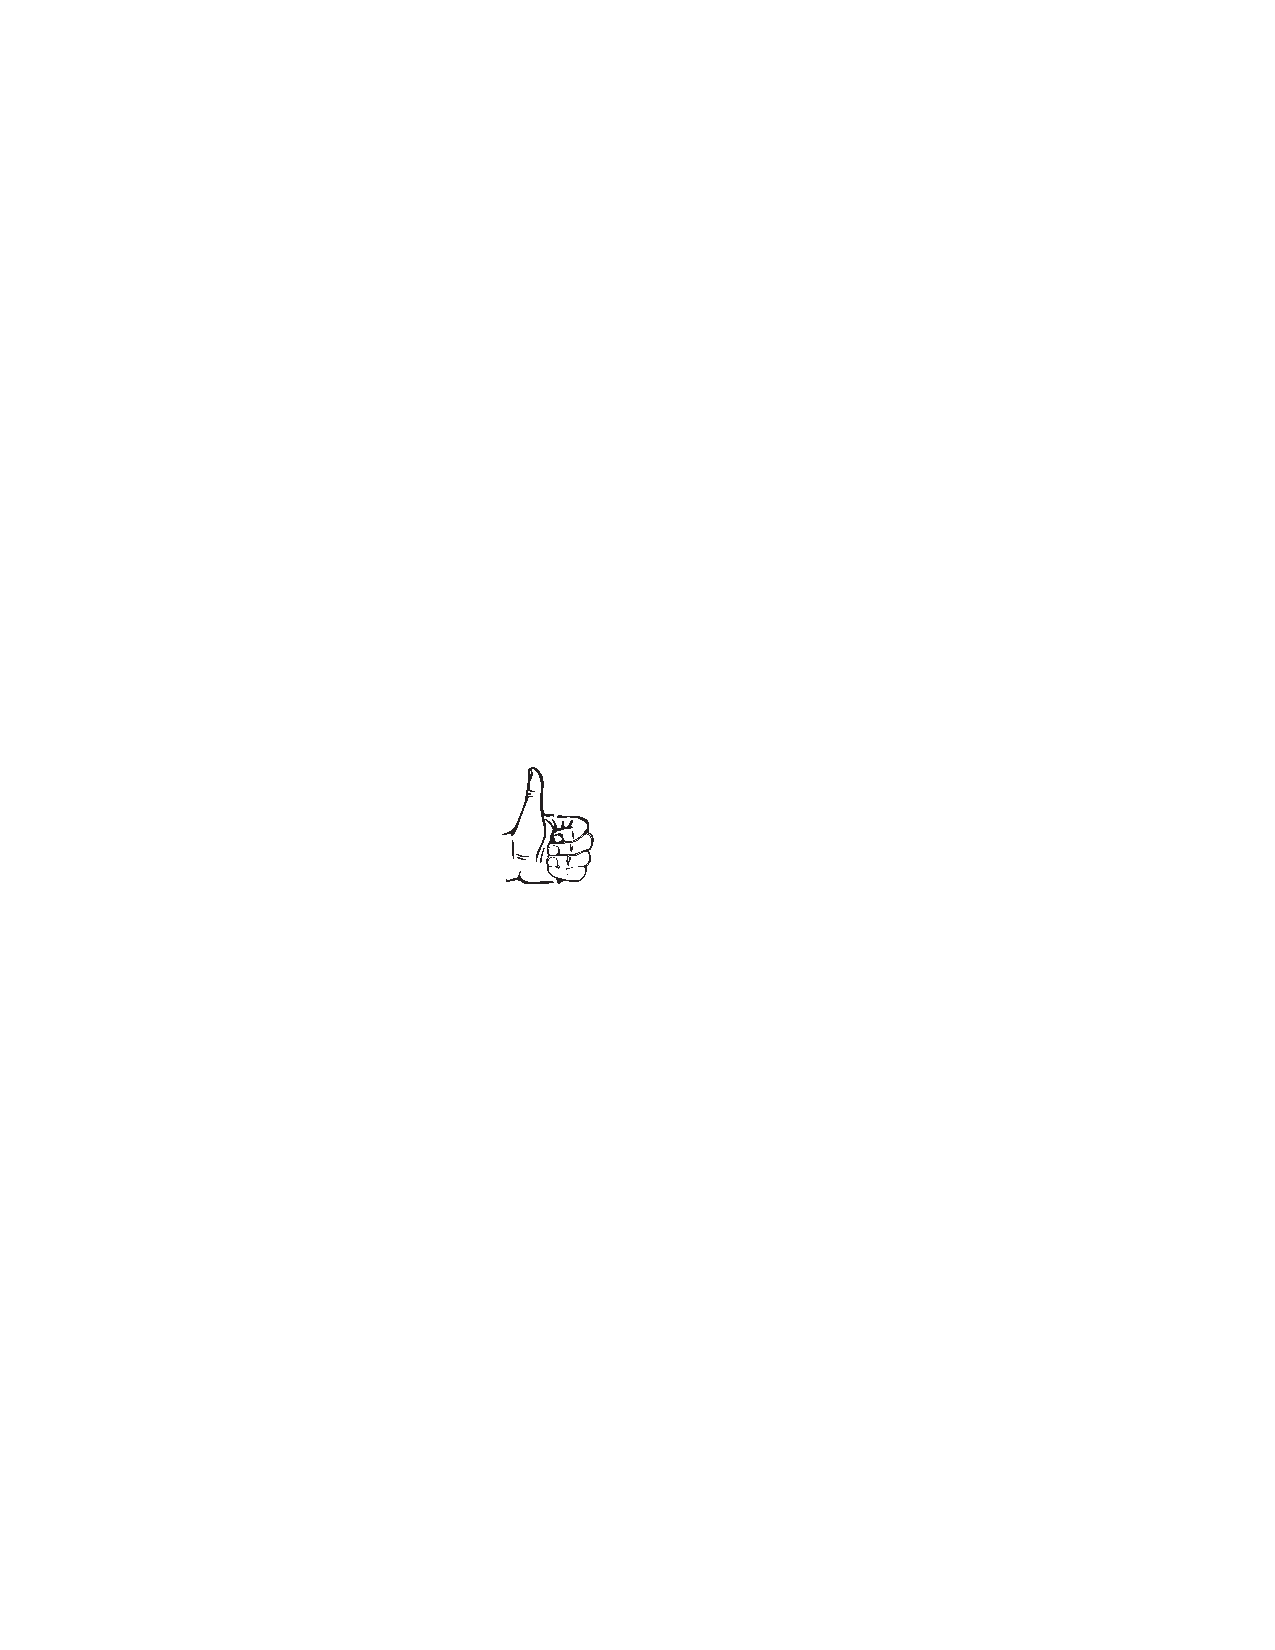
\includegraphics[width = 0.5in ]{pdf/"ch 08"/Louie} & \includegraphics[width = 0.5in ]{pdf/"ch 08"/Ralph} \\\hline
 chirality & left & right \\
 angle increases & clockwise & counterclockwise \\
 shading & red & green \\
 viewpoint & below $x-y$ plane & above $x-y$ plane
\end{tabular}
\end{center}
\caption[Chirality can be expressed in different ways]{Chirality can be expressed in different ways.}
\label{default}
\end{table}%


\endinput